\chapter{Methodology and Development Strategy}

\section{Agile-AI Hybrid Methodology}

The development of CloudForge AI required a sophisticated methodology that could accommodate both traditional software development practices and the unique challenges of artificial intelligence application development. Our approach combines proven Agile principles with AI-specific practices to create a comprehensive development framework.

\subsection{Methodological Foundation}

The CloudForge AI methodology is built upon four foundational pillars that ensure both development velocity and AI model quality:

\begin{sprintbox}{Agile Software Development Principles}
\begin{itemize}
    \item Iterative development with 2-week sprints
    \item Continuous stakeholder collaboration and feedback
    \item Adaptive planning and requirement evolution
    \item Working software delivery at regular intervals
    \item Cross-functional team collaboration
\end{itemize}
\end{sprintbox}

\begin{sprintbox}{Machine Learning Operations (MLOps)}
\begin{itemize}
    \item Experiment tracking and model versioning
    \item Automated model training and validation pipelines
    \item Continuous integration for ML models
    \item Model performance monitoring and drift detection
    \item A/B testing for model comparison and selection
\end{itemize}
\end{sprintbox}

\begin{sprintbox}{DevOps and Infrastructure as Code}
\begin{itemize}
    \item Containerized application deployment
    \item Infrastructure automation and version control
    \item Continuous deployment with automated rollbacks
    \item Comprehensive monitoring and alerting
    \item Security-first development practices
\end{itemize}
\end{sprintbox}

\begin{sprintbox}{Data-Driven Decision Making}
\begin{itemize}
    \item Metrics-based feature prioritization
    \item Performance benchmarking and optimization
    \item User behavior analysis and feedback integration
    \item Predictive analytics for project planning
    \item Continuous improvement through data analysis
\end{itemize}
\end{sprintbox}

\section{Sprint Planning and Execution Framework}

\subsection{Sprint Structure and Timeline}

Each CloudForge AI sprint follows a carefully orchestrated timeline designed to maximize productivity while ensuring comprehensive quality assurance:

\begin{figure}[H]
\centering
\begin{ganttchart}[
    hgrid,
    vgrid,
    time slot format=isodate,
    x unit=0.8cm,
    y unit title=0.8cm,
    y unit chart=0.8cm,
    title label font=\footnotesize,
    bar label font=\footnotesize,
    group label font=\footnotesize
]{2025-01-01}{2025-01-14}
    \gantttitlecalendar{day} \\
    \ganttgroup{Sprint Planning}{2025-01-01}{2025-01-02} \\
    \ganttbar{Backlog Refinement}{2025-01-01}{2025-01-01} \\
    \ganttbar{Sprint Planning Meeting}{2025-01-02}{2025-01-02} \\
    
    \ganttgroup{Development Phase}{2025-01-03}{2025-01-10} \\
    \ganttbar{Feature Implementation}{2025-01-03}{2025-01-08} \\
    \ganttbar{ML Model Development}{2025-01-03}{2025-01-07} \\
    \ganttbar{Unit Testing}{2025-01-06}{2025-01-10} \\
    
    \ganttgroup{Integration \& Testing}{2025-01-09}{2025-01-12} \\
    \ganttbar{Integration Testing}{2025-01-09}{2025-01-11} \\
    \ganttbar{Performance Testing}{2025-01-10}{2025-01-12} \\
    
    \ganttgroup{Review \& Retrospective}{2025-01-13}{2025-01-14} \\
    \ganttbar{Sprint Review}{2025-01-13}{2025-01-13} \\
    \ganttbar{Sprint Retrospective}{2025-01-14}{2025-01-14} \\
    
    \ganttlink{elem0}{elem3}
    \ganttlink{elem3}{elem6}
    \ganttlink{elem6}{elem9}
\end{ganttchart}
\caption{Standard Sprint Timeline (2-Week Cycle)}
\label{fig:sprint_timeline}
\end{figure}

\subsection{Sprint Planning Process}

The sprint planning process is divided into two distinct phases, each serving specific objectives:

\subsubsection{Sprint Planning Part I: What to Build}

\begin{enumerate}[leftmargin=*]
    \item \textbf{Product Owner Presentation}: Detailed presentation of prioritized user stories with business value justification
    \item \textbf{Acceptance Criteria Review}: Comprehensive discussion of user story acceptance criteria and edge cases
    \item \textbf{Technical Feasibility Assessment}: Engineering team evaluation of implementation complexity and dependencies
    \item \textbf{Sprint Goal Definition}: Collaborative definition of the sprint objective and success metrics
    \item \textbf{Capacity Planning}: Team velocity analysis and realistic commitment determination
\end{enumerate}

\subsubsection{Sprint Planning Part II: How to Build}

\begin{enumerate}[leftmargin=*]
    \item \textbf{Task Decomposition}: Breaking user stories into implementable tasks with clear deliverables
    \item \textbf{Technical Design Discussion}: Architecture decisions, API design, and integration approaches
    \item \textbf{ML Model Strategy}: Algorithm selection, training data requirements, and validation approaches
    \item \textbf{Testing Strategy Definition}: Comprehensive testing plan including unit, integration, and performance tests
    \item \textbf{Risk Assessment}: Identification of potential blockers and mitigation strategies
\end{enumerate}

\section{User Story Development and Management}

\subsection{User Story Template and Structure}

CloudForge AI user stories follow a standardized template that ensures clarity, testability, and alignment with business objectives:

\begin{tcolorbox}[colback=lightgray, colframe=primaryblue, title=User Story Template]
\textbf{As a} [user role] \\
\textbf{I want} [functionality] \\
\textbf{So that} [business value] \\

\textbf{Acceptance Criteria:}
\begin{itemize}
    \item Given [context] When [action] Then [expected outcome]
    \item Given [context] When [action] Then [expected outcome]
    \item Given [context] When [action] Then [expected outcome]
\end{itemize}

\textbf{Definition of Done:}
\begin{itemize}
    \item Code implemented and reviewed
    \item Unit tests written and passing
    \item Integration tests passing
    \item Documentation updated
    \item Performance benchmarks met
\end{itemize}
\end{tcolorbox}

\subsection{Story Prioritization Framework}

User stories are prioritized using a multi-criteria decision framework that balances business value, technical complexity, and strategic alignment:

\begin{table}[H]
\centering
\caption{Story Prioritization Criteria}
\begin{tabular}{|p{3cm}|p{2cm}|p{7cm}|}
\hline
\textbf{Criteria} & \textbf{Weight} & \textbf{Description} \\
\hline
Business Value & 40\% & Revenue impact, user satisfaction, competitive advantage \\
\hline
Strategic Alignment & 25\% & Platform vision alignment, long-term goals contribution \\
\hline
Technical Risk & 20\% & Implementation complexity, dependency management \\
\hline
User Impact & 15\% & Number of affected users, frequency of use \\
\hline
\end{tabular}
\end{table}

\section{Quality Assurance and Testing Methodology}

\subsection{Comprehensive Testing Strategy}

CloudForge AI employs a multi-layered testing approach that addresses both traditional software quality and AI-specific validation requirements:

\subsubsection{Traditional Software Testing}

\begin{description}[leftmargin=*]
    \item[Unit Testing] Individual component testing with 85\%+ code coverage requirement
    \item[Integration Testing] Component interaction validation and API contract testing
    \item[End-to-End Testing] Complete user journey validation using Cypress automation
    \item[Performance Testing] Load testing, stress testing, and scalability validation
    \item[Security Testing] Vulnerability scanning, penetration testing, and compliance validation
\end{description}

\subsubsection{AI-Specific Testing}

\begin{description}[leftmargin=*]
    \item[Model Validation Testing] Cross-validation, holdout testing, and statistical significance analysis
    \item[Data Quality Testing] Schema validation, data drift detection, and outlier identification
    \item[Prediction Accuracy Testing] Baseline comparison, A/B testing, and performance benchmarking
    \item[Robustness Testing] Edge case handling, input validation, and error recovery mechanisms
    \item[Ethical AI Testing] Bias detection, fairness assessment, and transparency validation
\end{description}

\subsection{Continuous Integration and Deployment Pipeline}

The CloudForge AI CI/CD pipeline ensures automated quality gates and reliable deployment processes:

\begin{figure}[H]
\centering
\begin{tikzpicture}[node distance=1.5cm, auto]
    \tikzstyle{stage} = [rectangle, rounded corners, minimum width=2.5cm, minimum height=1cm, text centered, draw=primaryblue, fill=lightgray, font=\small]
    \tikzstyle{gate} = [diamond, minimum width=1.5cm, minimum height=1cm, text centered, draw=secondaryblue, fill=white, font=\footnotesize]
    
    % CI/CD Stages
    \node [stage] (commit) {Code Commit};
    \node [stage, right of=commit, xshift=2cm] (build) {Build \& Test};
    \node [gate, right of=build, xshift=2cm] (quality) {Quality Gate};
    \node [stage, right of=quality, xshift=2cm] (deploy) {Deploy};
    \node [stage, right of=deploy, xshift=2cm] (monitor) {Monitor};
    
    % Feedback loops
    \draw [->] (commit) -- (build);
    \draw [->] (build) -- (quality);
    \draw [->] (quality) -- node[above] {Pass} (deploy);
    \draw [->] (deploy) -- (monitor);
    \draw [->] (quality) -- ++ (0,-2) -| node[below] {Fail} (commit);
    \draw [->] (monitor) -- ++ (0,-2.5) -| (commit);
\end{tikzpicture}
\caption{Continuous Integration and Deployment Pipeline}
\label{fig:cicd_pipeline}
\end{figure}

\section{Performance Monitoring and Optimization}

\subsection{Key Performance Indicators (KPIs)}

CloudForge AI tracks comprehensive performance metrics across multiple dimensions:

\begin{table}[H]
\centering
\caption{Performance Monitoring KPIs}
\begin{tabular}{|p{3cm}|p{3cm}|p{2cm}|p{4cm}|}
\hline
\textbf{Category} & \textbf{Metric} & \textbf{Target} & \textbf{Monitoring Method} \\
\hline
\multirow{3}{*}{Application Performance} & Response Time & < 50ms & Real-time APM monitoring \\
\cline{2-4}
 & Throughput & > 1000 RPS & Load balancer metrics \\
\cline{2-4}
 & Error Rate & < 0.1\% & Application logs analysis \\
\hline
\multirow{3}{*}{AI Model Performance} & Prediction Accuracy & > 80\% & Model validation pipeline \\
\cline{2-4}
 & Inference Time & < 100ms & Model serving metrics \\
\cline{2-4}
 & Model Drift & < 5\% & Statistical monitoring \\
\hline
\multirow{3}{*}{Infrastructure Performance} & CPU Utilization & < 70\% & Kubernetes metrics \\
\cline{2-4}
 & Memory Usage & < 80\% & Container monitoring \\
\cline{2-4}
 & Disk I/O & < 80\% & System metrics \\
\hline
\end{tabular}
\end{table}

\subsection{Optimization Strategies}

Performance optimization follows a systematic approach based on measurement, analysis, and iterative improvement:

\begin{enumerate}[leftmargin=*]
    \item \textbf{Baseline Establishment}: Comprehensive performance baseline measurement across all system components
    \item \textbf{Bottleneck Identification}: Systematic analysis using profiling tools and performance monitoring
    \item \textbf{Optimization Implementation}: Targeted improvements based on identified bottlenecks
    \item \textbf{Impact Validation}: Rigorous testing to validate optimization effectiveness
    \item \textbf{Continuous Monitoring}: Ongoing performance tracking and alert-based optimization triggers
\end{enumerate}

\section{Risk Management and Mitigation}

\subsection{Risk Assessment Framework}

CloudForge AI employs a comprehensive risk assessment framework that evaluates both likelihood and impact of potential issues:

\begin{figure}[H]
\centering
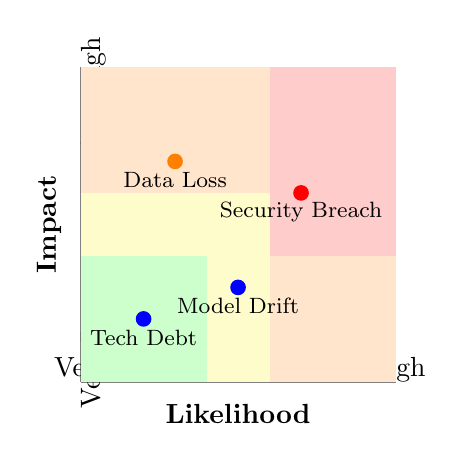
\begin{tikzpicture}[scale=0.8]
    % Risk matrix
    \draw[step=1cm,gray,very thin] (0,0) grid (5,5);
    
    % Labels
    \node at (2.5,-0.5) {\textbf{Likelihood}};
    \node at (-0.5,2.5) [rotate=90] {\textbf{Impact}};
    
    % Axis labels
    \node at (0.5,0.2) {Very Low};
    \node at (1.5,0.2) {Low};
    \node at (2.5,0.2) {Medium};
    \node at (3.5,0.2) {High};
    \node at (4.5,0.2) {Very High};
    
    \node at (0.2,0.5) [rotate=90] {Very Low};
    \node at (0.2,1.5) [rotate=90] {Low};
    \node at (0.2,2.5) [rotate=90] {Medium};
    \node at (0.2,3.5) [rotate=90] {High};
    \node at (0.2,4.5) [rotate=90] {Very High};
    
    % Risk zones
    \fill[green!20] (0,0) rectangle (2,2);
    \fill[yellow!20] (2,0) rectangle (3,3);
    \fill[yellow!20] (0,2) rectangle (2,3);
    \fill[orange!20] (3,0) rectangle (5,2);
    \fill[orange!20] (2,3) rectangle (3,5);
    \fill[orange!20] (0,3) rectangle (2,5);
    \fill[red!20] (3,2) rectangle (5,5);
    
    % Risk items
    \node at (1,1) [circle, fill=blue, inner sep=2pt] {};
    \node at (1,0.7) {\footnotesize Tech Debt};
    
    \node at (2.5,1.5) [circle, fill=blue, inner sep=2pt] {};
    \node at (2.5,1.2) {\footnotesize Model Drift};
    
    \node at (3.5,3) [circle, fill=red, inner sep=2pt] {};
    \node at (3.5,2.7) {\footnotesize Security Breach};
    
    \node at (1.5,3.5) [circle, fill=orange, inner sep=2pt] {};
    \node at (1.5,3.2) {\footnotesize Data Loss};
\end{tikzpicture}
\caption{Risk Assessment Matrix}
\label{fig:risk_matrix}
\end{figure}

\subsection{Mitigation Strategies}

For each identified risk category, specific mitigation strategies are implemented:

\begin{description}[leftmargin=*]
    \item[Technical Risks] Code reviews, automated testing, redundant architectures, and disaster recovery planning
    \item[Operational Risks] Monitoring and alerting systems, incident response procedures, and capacity planning
    \item[Security Risks] Security audits, penetration testing, compliance frameworks, and access controls
    \item[Business Risks] Stakeholder communication, change management processes, and alternative solution planning
\end{description}

This comprehensive methodology ensures that CloudForge AI development maintains high quality standards while adapting to the unique challenges of AI application development. The subsequent sprint chapters will demonstrate the practical application of these methodological principles in real-world development scenarios.